% Тип документа
\documentclass[a4paper,12pt]{extarticle}

% Шрифты, кодировки, символьные таблицы, переносы
\usepackage{cmap}
\usepackage[T2A]{fontenc}
\usepackage[utf8x]{inputenc}
\usepackage[russian]{babel}

% Это пакет -- хитрый пакет, он нужен но не нужен
\usepackage[mode=buildnew]{standalone}

\usepackage
	{
		% Дополнения Американского математического общества (AMS)
		amssymb,
		amsfonts,
		amsmath,
		amsthm,
		% misccorr,
		% 
		% Графики и рисунки
		wrapfig,
		graphicx,
		subcaption,
		float,
		tikz,
		tikz-3dplot,
		caption,
		csvsimple,
		color,
		booktabs,
		pgfplots,
		pgfplotstable,
		geometry,
		% 
		% Таблицы, списки
		makecell,
		multirow,
		indentfirst,
		%
		% Интегралы и прочие обозначения
		ulem,
		esint,
		esdiff,
		% 
		% Колонтитулы
		fancyhdr,
	}  


% Обводка текста в TikZ
\usepackage[outline]{contour}

% Увеличенный межстрочный интервал, французские пробелы
\linespread{1.3} 
\frenchspacing 

 
\usetikzlibrary
	{
		decorations.pathreplacing,
		decorations.pathmorphing,
		patterns,
		calc,
		scopes,
		arrows,
		fadings,
		through,
		shapes.misc,
		arrows.meta,
		3d,
		quotes,
		angles,
		babel
	}


\tikzset{
	force/.style=	{
		>=latex,
		draw=blue,
		fill=blue,
				 	}, 
	%				 	
	axis/.style=	{
		densely dashed,
		blue,
		line width=1pt,
		font=\small,
					},
	%
	th/.style=	{
		line width=1pt},
	%
	acceleration/.style={
		>=open triangle 60,
		draw=magenta,
		fill=magenta,
					},
	%
	inforce/.style=	{
		force,
		double equal sign distance=2pt,
					},
	%
	interface/.style={
		pattern = north east lines, 
		draw    = none, 
		pattern color=gray!60,
					},
	cross/.style=	{
		cross out, 
		draw=black, 
		minimum size=2*(#1-\pgflinewidth), 
		inner sep=0pt, outer sep=0pt,
					},
	%
	cargo/.style=	{
		rectangle, 
		fill=black!70, 
		inner sep=2.5mm,
					},
	%
	caption/.style= {
		midway,
		fill=white!20, 
		opacity=0.9
					},
	%
	}

\newenvironment{tikzpict}
    {
	    \begin{figure}[htbp]
		\centering
		\begin{tikzpicture}
    }
    { 
		\end{tikzpicture}
		% \caption{caption}
		% \label{fig:label}
		\end{figure}
    }


\newcommand{\vbLabel}[3]{\draw ($(#1,#2)+(0,5pt)$) -- ($(#1,#2)-(0,5pt)$) node[below]{#3}}
\newcommand{\vaLabel}[3]{\draw ($(#1,#2)+(0,5pt)$) node[above]{#3} -- ($(#1,#2)-(0,5pt)$) }

\newcommand{\hrLabel}[3]{\draw ($(#1,#2)+(5pt,0)$) -- ($(#1,#2)-(5pt,0)$) node[right, xshift=1em]{#3}}
\newcommand{\hlLabel}[3]{\draw ($(#1,#2)+(5pt,0)$) node[left, xshift=-1em]{#3} -- ($(#1,#2)-(5pt,0)$) }



\newcommand\zi{^{\,*}_i}
\newcommand\sumn{\sum_{i=1}^{N}}

\tikzset{
	coordsys/.style={scale=1.8,x={(1.1cm,-0cm)},y={(0.5cm,1cm)}, z={(0cm,0.8cm)}},
	coordsys/.style={scale=1.5,x={(0cm,0cm)},y={(1cm,0cm)}, z={(0cm,1cm)}}, 
	coordsys/.style={scale=1.5,x={(1cm,0cm)},y={(0cm,1cm)}, z={(0cm,0cm)}}, 
}

\usepgfplotslibrary{units}


% Draw line annotation
% Input:
%   #1 Line offset (optional)
%   #2 Line angle
%   #3 Line length
%   #5 Line label
% Example:
%   \lineann[1]{30}{2}{$L_1$}

\newcommand{\lineann}[4][0.5]{%
    \begin{scope}[rotate=#2, blue,inner sep=2pt, ]
        \draw[dashed, blue!40] (0,0) -- +(0,#1)
            node [coordinate, near end] (a) {};
        \draw[dashed, blue!40] (#3,0) -- +(0,#1)
            node [coordinate, near end] (b) {};
        \draw[|<->|] (a) -- node[fill=white, scale=0.8] {#4} (b);
    \end{scope}
}

\newcommand{\lineannn}[4][0.5]{%
    \begin{scope}[rotate=#2, blue,inner sep=2pt, ]
        \draw[dashed, blue!40] (0,0) -- +(0,#1)
            node [coordinate, near end] (a) {};
        \draw[dashed, blue!40] (#3,0) -- +(0,#1)
            node [coordinate, near end] (b) {};
        % \draw[color=white, color=blue] (a) -- node[fill=white, scale=0.8] {#4} (b);
        \draw[->|] (a)++(-0.3,0) -- (a);
        \draw[->|] (b)++(0.3,0) coordinate (xx) -- (b);
        \draw (xx) node[fill=white, scale=0.8, right] {#4};
    \end{scope}
}

% Круговая стрелка относительно центра (дуга из центра)
\tikzset{
  pics/carc/.style args={#1:#2:#3}{
    code={
      \draw[pic actions] (#1:#3) arc(#1:#2:#3);
    }
  },
  dash/.style={
  	dash pattern=on 5mm off 5mm
  }
}

% Среднее <#1>
\newcommand{\mean}[1]{\langle#1\rangle}

\pgfplotsset{
    % most recent feature set of pgfplots
    compat=newest,
}

% const прямым шрифтом
\newcommand\ct[1]{\text{\rmfamily\upshape #1}}
\newcommand*{\const}{\ct{const}}


\usepackage[europeanresistors,americaninductors]{circuitikz}

% Style to select only points from #1 to #2 (inclusive)
\pgfplotsset{select/.style 2 args={
    x filter/.code={
        \ifnum\coordindex<#1\def\pgfmathresult{}\fi
        \ifnum\coordindex>#2\def\pgfmathresult{}\fi
    }
}}


\usepackage{array}



%%%%%%%%%%%%%%%%%%%%%%%%%%%%%%%%%%%%%%%%%%%%%%%%%
\makeatletter
\newif\if@gather@prefix 
\preto\place@tag@gather{% 
  \if@gather@prefix\iftagsleft@ 
    \kern-\gdisplaywidth@ 
    \rlap{\gather@prefix}% 
    \kern\gdisplaywidth@ 
  \fi\fi 
} 
\appto\place@tag@gather{% 
  \if@gather@prefix\iftagsleft@\else 
    \kern-\displaywidth 
    \rlap{\gather@prefix}% 
    \kern\displaywidth 
  \fi\fi 
  \global\@gather@prefixfalse 
} 
\preto\place@tag{% 
  \if@gather@prefix\iftagsleft@ 
    \kern-\gdisplaywidth@ 
    \rlap{\gather@prefix}% 
    \kern\displaywidth@ 
  \fi\fi 
} 
\appto\place@tag{% 
  \if@gather@prefix\iftagsleft@\else 
    \kern-\displaywidth 
    \rlap{\gather@prefix}% 
    \kern\displaywidth 
  \fi\fi 
  \global\@gather@prefixfalse 
} 
\newcommand*{\beforetext}[1]{% 
  \ifmeasuring@\else
  \gdef\gather@prefix{#1}% 
  \global\@gather@prefixtrue 
  \fi
} 
\makeatother
%%%%%%%%%%%%%%%%%%%%%%%%%%%%%%%%%%%%%%%%%%%%%%%%%

\geometry		
	{
		left			=	2cm,
		right 			=	2cm,
		top 			=	3cm,
		bottom 			=	3cm,
		bindingoffset	=	0cm
	}

%%%%%%%%%%%%%%%%%%%%%%%%%%%%%%%%%%%%%%%%%%%%%%%%%%%%%%%%%%%%%%%%%%%%%%%%%%%%%%%



	%применим колонтитул к стилю страницы
\pagestyle{fancy} 
	%очистим "шапку" страницы
\fancyhead{} 
	%слева сверху на четных и справа на нечетных
\fancyhead[R]{\labauthors} 
	%справа сверху на четных и слева на нечетных
\fancyhead[L]{Отчёт по лабораторной работе №\labnumber} 
	%очистим "подвал" страницы
\fancyfoot{} 
	% номер страницы в нижнем колинтуле в центре
\fancyfoot[C]{\thepage} 

%%%%%%%%%%%%%%%%%%%%%%%%%%%%%%%%%%%%%%%%%%%%%%%%%%%%%%%%%%%%%%%%%%%%%%%%%%%%%%%

\renewcommand{\contentsname}{Оглавление}

\usepackage{tocloft}
% \renewcommand{\cftpartleader}{\cftdotfill{\cftdotsep}} % for parts
% \renewcommand{\cftsectiondotsep}{\cftdotsep}% Chapters should use dots in ToC
\renewcommand{\cftsecleader}{\cftdotfill{\cftdotsep}}
%\renewcommand{\cftsecleader}{\cftdotfill{\cftdotsep}} % for sections, if you really want! (It is default in report and book class (So you may not need it).
% ---------
% \newcommand{\cftchapaftersnum}{.}%
% \usepackage{titlesec}
% \titlelabel{\thetitle.\quad}
\usepackage{secdot}
\sectiondot{subsection}
\usepackage{setspace}

\begin{document}

\def\labauthors{Понур К.А., Сарафанов Ф.Г., Сидоров Д.А.}
\def\labgroup{420}
\def\labnumber{217}
\def\labtheme{Исследование колебательных процессов в электрическом контуре}
\renewcommand{\vec}{\mathbf}
\renewcommand{\Re}{\operatorname{Re}}
\renewcommand{\Im}{\operatorname{Im}}
\renewcommand{\phi}{\varphi}
\renewcommand{\kappa}{\varkappa}
\renewcommand{\hat}{\widehat}
%%%%%%%%%%%%%%%%%%%%%%%%%%%%%%%%%%%%%%%%%%%%%%%%%%%%%%%%%%%%%%%%%%%%%%%%%%%%%%%
\begin{titlepage}

\begin{center}

{\small\textsc{Нижегородский государственный университет имени Н.\,И. Лобачевского}}
\vskip 1pt \hrule \vskip 3pt
{\small\textsc{Радиофизический факультет}}

\vfill

{\Large Отчет по лабораторной работе №\labnumber\vskip 12pt\bfseries \labtheme}
	
\end{center}

\vfill
	
\begin{flushright}
	{Выполнили студенты \labgroup\ группы\\ \labauthors}%\vskip 12pt Принял:\\ Менсов С.\,Н.}
\end{flushright}
	
\vfill
	
\begin{center}
	Нижний Новгород, \the\year
\end{center}

\end{titlepage}


%%%%%%%%%%%%%%%%%%%%%%%%%%%%%%%%%%%%%%%%%%%%%%%%%%%%%%%%%%%%%%%%%%%%%%%%%%%%%%%
\begin{spacing}{1.2}
\tableofcontents
\end{spacing}
% \setstretch{1.2}
\newpage
%%%%%%%%%%%%%%%%%%%%%%%%%%%%%%%%%%%%%%%%%%%%%%%%%%%%%%%%%%%%%%%%%%%%%%%%%%%%%%%


\section{}
\subsection{Введение}
Цель работы -- экспериментальное исследование колебатель
ных процессов в линейном осцилляторе с потерями. В качестве осциллятора используется электрический
контур, состоящий из последовательно соединенных
катушки индуктивности $L$,
конденсатора $C$, резистора $R$
и внешнего источника ЭДС $\varepsilon$.
Дифференциальное уравнение, описывающее процессы в исследуемом контуре, имеет следующий вид:
\begin{equation}
	q''+2\delta q'+\omega_0 q=f(t),
\end{equation}
где q--заряд на конденсаторе, $\delta=\frac{R}{2L}$--коэффициент затухания, $\omega_0=\frac{1}{\sqrt{LC}}$--собственная частота контура, $f(t)=\frac{\varepsilon(t)}{L}$-- "вынуждающая сила", $\varepsilon(t)$-- внешняя ЭДС.
 

С математической точки зрения уравнение (1) является неоднородным линейным дифференциальным уравнением 2-го порядка с постоянными коэффициентами. Решение такого уравнения, как известно, можно представить в виде суммы общего решения соответствующего однородного уравнения
\begin{equation}
	\ddot{q}+2\delta \dot{q}+\omega_0 q=0
\end{equation}
и частного решения неоднородного. Уравнение (2) описывает поведение осциллятора в отсутствие внешней ЭДС, т.е. так называемые собственные (свободные) колебания, а частное решение неоднородного уравнения (1) (в случае периодического внешнего воздействия) - вынужденные колебания. Исследованию этих двух режимов и уделяется основное внимание в работе. Кроме того, лабораторная установка позволяет наблюдать некоторые переходные процессы, в частности процессы установления колебаний.
\begin{figure}[h!]
	\centering
    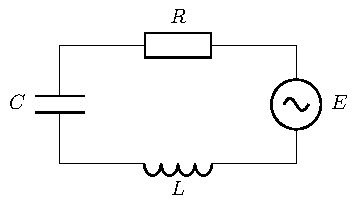
\includegraphics[]{chem/rcle}
    \caption{}
    \label{chem:rcle}
\end{figure}

%%%%%%%%%%%%%%%%%%%%%%%%%%%%%%%%%%%%%%%%%%%%%%%%%%%%%%%%%%%%%%%%%%%%%%%%%%%%%%%
\subsection{Собственные колебания в электрическом контуре}
При анализе решения уравнения (2) удобно выделить три случая: $\delta > \omega_0$,$\delta < \omega_0$ ,$\delta = \omega_0$.
В случае достаточно слабого затухания, когда $\delta < \omega_0$ общее решение уравнения (2) можно представить в виде
\begin{equation}
	q=A_0 e^{-\delta t}\cos(\omega_s t+\phi),
\end{equation}
где $\omega_s=\sqrt{\omega_0^2-\delta^2}$, а $A_0$ и $\phi$ -- произвольные постоянные, определяемые из начальных условий.
Процесс вида (3) называют затухающими квазигармоническими колебаниями. Если $\delta<<\omega_0$, то выличину $A(t)=A_0e^{-\delta t}$ можно считать медленно меняющейся амплитудой, а 
$T=\frac{2\pi}{\omega_s}$-- "периодом" этих колебаний.
В отсутстввие затухания $(\delta=0)$ решение уравнения (2) можно представить в виде
\begin{equation}
	q=A_1e^{\alpha_1 t}+A_2e^{\alpha_2 t},
\end{equation}
где $A_1$ и $A_2$ зависят от начальных условий, а 
\begin{equation}
	\alpha_{1,2}=-\delta+-\sqrt{\delta^2-\omega_0^2}
\end{equation}

Процесс, описываемый формулой (4), называется апериодическим.


Условие $\delta=\omega_0$ определяет критический режим колебаний, а соответствующее этому условию сопротивление называется кри 
тическим сопротивлением контура: $R_{\text{кр}}=2\sqrt{\frac{L}{C}}$. На практике используется также характеристическое (волновое) сопротивление 
контура: $\rho=\sqrt{\frac{L}{C}}$.

%%%%%%%%%%%%%%%%%%%%%%%%%%%%%%%%%%%%%%%%%%%%%%%%%%%%%%%%%%%%%%%%%%%%%%%%%%%%%%%
\subsection{Декремент затухания. Добротность}
Логарифмическим декрементом затухания $d$ называется логарифм отношения значений заряда $q$ на пластинах конденсатора в двух последовательных ($n$-ом и ($n+1$)-ом) максимумах:
\begin{equation}
	d=\ln{\frac{q_n}{q_{n+1}}}=\delta T
\end{equation}
Поскольку, как видно из выражения (3), $\delta$ есть величина, обратная промежутку времени $\tau$, за которое амплитуда колебаний спадает в $e$ раз, то можно определить число колебаний $N$. совершившихся за это время:
\begin{equation}
	N=\frac{\tau}{T}=
		\frac{1}{\delta T}=
			\frac{1}{d}
\end{equation}

Таким образом, логарифмический декремент затухания $d$ есть величина, обратная числу колебаний N. в течение которых амплитуда колебаний уменьшается в $e$ раз.
Часто для характеристики затухания удобнее использовать не N. а величину в $\pi$ раз большую - добротность контура $Q=\pi N$.
 
При малом затухании ($\delta \ll \omega_0$) частота собственных колебаний 
$\omega_s=\sqrt{\omega_0^2 - \delta^2}=\omega_0$. 
При этом добротность контура и его
логарифмический декремент затухания можно выразить через параметры контура L, С, R следующим образом:
\begin{equation}
	d=\frac{\pi R}{\omega_0 L}=\pi RC\omega_0=\pi R\sqrt{\frac{C}{L}}
\end{equation}
\begin{equation}
	Q=\frac{\omega_0 L}{R}=\frac{1}{RC\omega_0}=\frac{1}{R}\sqrt{\frac{L}{C}}
\end{equation}

Необходимо иметь в виду, что во всех этих выражениях под следует понимать сопротивление, эквивалентное всем потерям в контуре. Дополнительные потери при прохождении переменного тока могут быть вызваны гистерезисом и токами Фуко в сердечнике катушки индуктивности, токами утечки и процессами поляризации в диэлектрике конденсатора.
%%%%%%%%%%%%%%%%%%%%%%%%%%%%%%%%%%%%%%%%%%%%%%%%%%%%%%%%%%%%%%%%%%%%%%%%%%%%%%%
\subsection{Фазовая плоскость} % (fold)

Процессы в колебательном контуре удобно изображать на так называемой фазовой плоскости, где по оси абсцисс откладывают заряд $q$, а по оси ординат величину, пропорциональную току.
например $\frac{\dot{q}}{\omega_0}$ (это величины одной размерности). Каждому
состоянию колебательного контура, характеризуемому мгновенными значениями $q$ и $\dot{q}$, соответствует точка на фазовой плоскости (изображающая точка). Изменение состояния вызывает перемещение изображающей точки по фазовой плоскости. Линия, описываемая изображающей точкой, называется фазовой траекторией. Совокупности движений с разными начальными условиями соответствует семейство фазовых траекторий. Например, гармоническим колебаниям в контуре без затухания  на фазовой плоскости соответствует семейство окружностей с общим центром в начале координат. Свободные затухающие колебания в контуре изображаются фазовыми траекториями в виде скручивающихся к началу координат спиралей.
%%%%%%%%%%%%%%%%%%%%%%%%%%%%%%%%%%%%%%%%%%%%%%%%%%%%%%%%%%%%%%%%%%%%%%%%%%%%%%%
\subsection{Вынужденные колебания в электрическом контуре} % (fold)
Колебания в контуре под действием внешней гармонической силы описывается уравнением
\begin{equation}
	\ddot{q}+2\delta\dot{q}+\omega_0^2 q= F_0\cos{\omega t}
\end{equation}
Решение этого уравнения, соответствующее установившемуся режиму, имеет вид
\begin{equation}
	q(t)=B(\omega)\cos{\omega t+\psi},
\end{equation}
где амплитуда $B(\omega)$ и фаза $\psi$ определяются следующим образом:
\begin{equation}
	B(\omega)=\frac{F_0}{\sqrt{(\omega^2-\omega_0^2)^2+4\delta^2\omega^2}}
\end{equation}
\begin{equation}
	\tan{\psi}=\frac{2\delta\omega}{\omega^2-\omega_0^2}
\end{equation}
	Используя формулы (11), (12), (13) и учитывая, что $F-0=\frac{\varepsilon_0}{L}$
Нетрудно получить выражения для амплитуды тока в контуре
\begin{equation}
	I_0=\omega B(\omega)=\frac{\varepsilon_0}{\sqrt{R^2+(\omega L-\frac{1}{\omega C})^2}}
\end{equation}
и для амплитуд напряжений на отдельных элементах контура
\begin{equation}
	U_L=I_0\omega L=\frac{\omega L\varepsilon_0}{\sqrt{R^2+(\omega L-\frac{1}{\omega C})^2}}
\end{equation}
\begin{equation}
	U_C=\frac{I_0}{\omega C}=\frac{\varepsilon_0}{\sqrt{R^2+(\omega L-\frac{1}{\omega C})^2}}
\end{equation}
\begin{equation}
	U_R=I_0R=\frac{\varepsilon_0R}{\sqrt{R^2+(\omega L-\frac{1}{\omega C})^2}}
\end{equation}

%%%%%%%%%%%%%%%%%%%%%%%%%%%%%%%%%%%%%%%%%%%%%%%%%%%%%%%%%%%%%%%%%%%%%%%%%%%%%%%
\subsection{Резонансные кривые}
\begin{center}
Резонансная кривая для индуктивности
\end{center}
\begin{equation}
	U_L=\frac{\omega L\varepsilon_0}
			{\sqrt{R^2+(\omega L-\frac{1}{\omega C})^2}}=
		\frac{\omega \varepsilon_0}
			{\sqrt{(\frac{R}{L})^2+(\omega -\frac{1}{\omega LC})^2}}=
		\frac{\omega \varepsilon_0}
			{\sqrt{(\frac{\omega_0}{Q})^2+(\omega -\frac{\omega_0^2}{\omega})^2}}
		\end{equation}
\begin{equation}
	U_L=\frac{\omega^2 \varepsilon_0}{\sqrt{\omega^2(\frac{\omega_0}{Q})^2+(\omega^2 -\omega_0^2)^2}}			
\end{equation}			


\begin{center}
Резонансная кривая для конденсатора
\end{center}

\begin{equation}
	U_C=\frac{\varepsilon_0}{\sqrt{R^2+(\omega L-\frac{1}{\omega C})^2}}=
		=\frac{\varepsilon_0\omega_0 Q}
			{\omega \sqrt{1+\frac{\omega^2}{\omega_0^2}(\omega-\frac{\omega_0^2}{\omega})^2}}
		=\frac{\varepsilon_0\omega_0^2}{\sqrt{\frac{\omega_0^2\omega^2}{Q^2}+(\omega^2-\omega_0^2)^2}}
\end{equation}

\begin{center}
Резонансная кривая для резистора
\end{center}
\begin{equation}
	U_R=\frac{\varepsilon_0\omega\omega_0}{\sqrt{\omega^2\omega_0^2+Q^2(\omega^2-\omega_0^2)^2}}
\end{equation}
Отсюда путем дифференцирования найдены максимумы резонансных  кривых и резонансные частоты:
\begin{equation}
	U_L^*=\frac{\varepsilon_0}{\sqrt{\frac{1}{Q^2}-\frac{1}{4Q^2}}}
\end{equation}
\begin{equation}
	\omega^*_L=\frac{\omega_0}{\sqrt{1-\frac{1}{2Q^2}}}
\end{equation}

\begin{equation}
	U_C^*=\frac{\varepsilon_0 Q}{\sqrt{1-\frac{1}{4Q^2}}}
\end{equation}
\begin{equation}
	\omega^*_C=\frac{\omega_0}{\sqrt{2}Q}\sqrt{2Q^2-1}
\end{equation}
\begin{equation}
		U_R^*=\varepsilon_0
\end{equation}	
\begin{equation}
		\omega_R^*=\omega_0
\end{equation}
\newpage

\section{Экспериментальная часть}
\subsection{Исследование свободных колебаний}
\subsubsection{Декремент затухания и добротность контура}
На установке рассмотрены осциллограммы $U_c(t)$ и $I(t)$ при нескольких сопротивлениях контура $R$. 

% Нашли период собственных колебаний контура и декремент затухания d для различных R
Получили декремент затухания $d$ для различных $R$:
\begin{figure}[H]
	\centering
	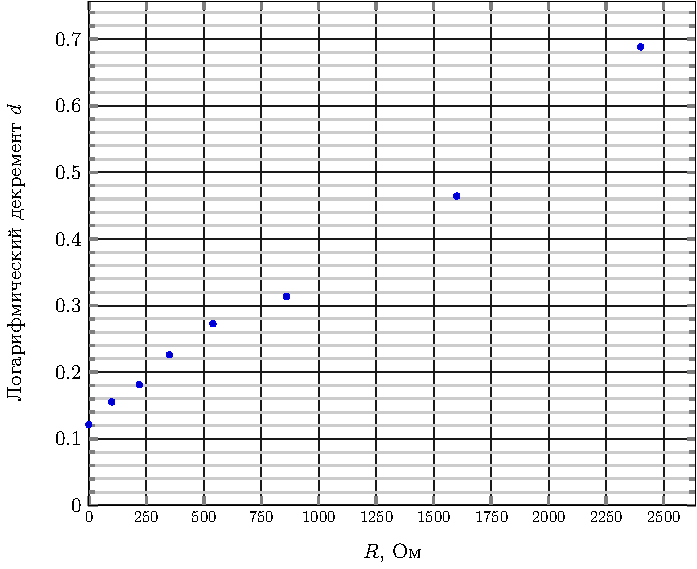
\includegraphics[]{plot/1c}
	\caption{Зависимость декремента затухания от сопротивления контура}
	\label{fig:figure1}
\end{figure}

Из эксперимента получили значение $L$ при $R=2400$ Ом:%
\begin{equation}
	L={R \over 2\delta}=\frac{RT}{2d}=\frac{2400 \cdot 0.4\cdot10^{-3}}{2\cdot0.688}= 0.708 \text{ Гн}
\end{equation}
Откуда можно вычислить критическое сопротивление контура:
\begin{equation}
	R_{k}=2\frac{L}{C}= 20407 \text{ Ом} \approx 20 \text{ кОм}
\end{equation}
Коэффициент затухания:
\begin{equation}
	\delta=\frac{R}{2L}=1694.91 \text{ рад/с}
\end{equation}
И добротность:
\begin{equation}
	Q=\frac{1}{R}\sqrt\frac{L}{C}=4.25
\end{equation}
% Построили графики зависимости $Т$ и $d$ от $R$.
% По выполненным измерениям рассчитать добротность контура О и коэффициент затухания 5 для одного из значений R. 

% Вычислить индуктивность и критическое сопротивление контура.
\subsubsection{Фазовые траектории при различных $R$}

\begin{figure}[H]
	\centering
	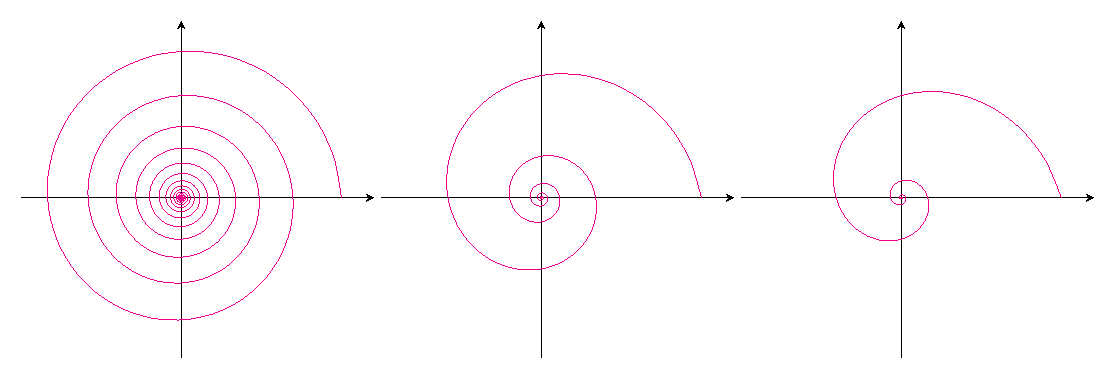
\includegraphics[]{plot/1e}
	\caption{Фазовые траектории}
	\label{fig:figure2}
\end{figure}


\subsection{Исследование вынужденных колебаний}
\begin{figure}[H]
	\centering
	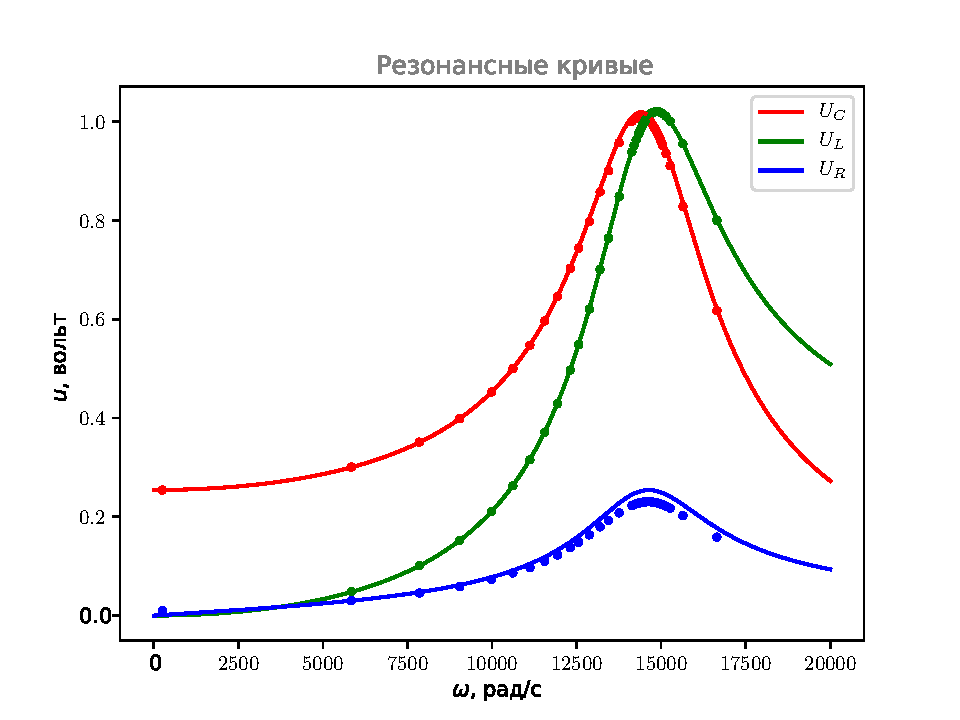
\includegraphics[width=0.86\linewidth]{plot/r2400}
	% \caption{Фазовые траектории}
	\label{fig:figure3}
\end{figure}
\begin{figure}[H]
	\centering
	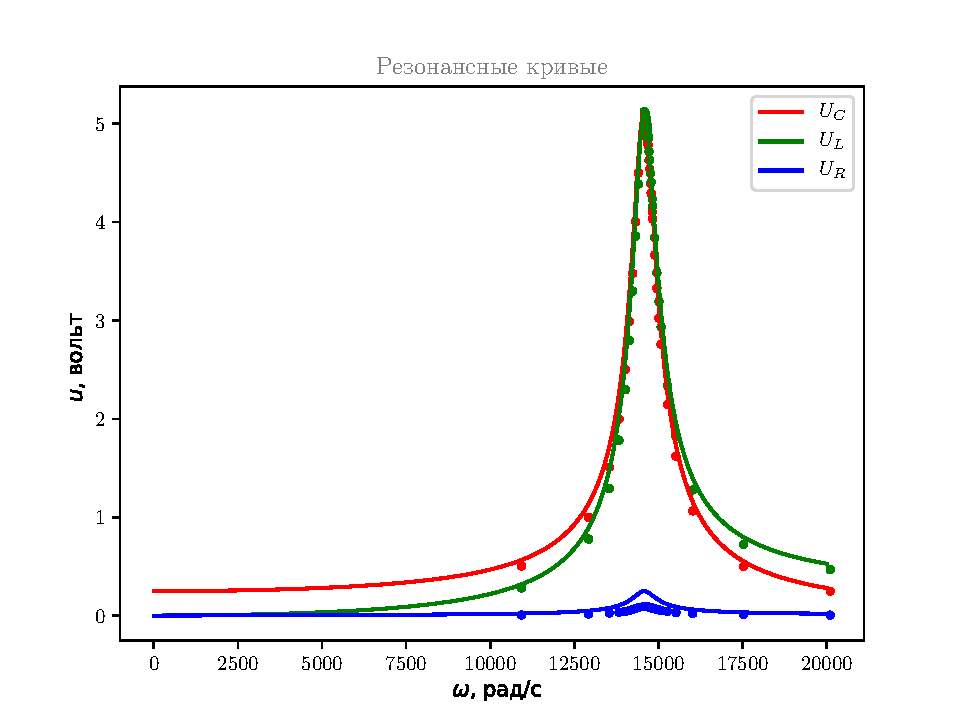
\includegraphics[width=0.86\linewidth]{plot/r100}
	% \caption{Фазовые траектории}
	\label{fig:figure4}
\end{figure}

При значении $R=100$ Ом получены следующие данные:
\begin{equation}
	\nu_0=\nu_0^C=\nu_0^R=2330 \text{ Гц}
\end{equation}
При значении $R=2400$ Ом получены следующие данные:
\begin{gather}
	\nu_0=2330 \text{ Гц}\\
	\nu_0^C=2293 \text{ Гц}\\
	\nu_0^R=2369 \text{ Гц}
\end{gather}
Из графика $R=2400$ Ом рассчитываются (считая точно известной ёмкость конденсатора)
\begin{gather}
	R=2524.94 \text{ Ом}\\
	L=0.686 \text{ Гн}
\end{gather}

Можно рассчитать добротность контура тремя способами.

Считая известными параметры установки:
\begin{equation}
	Q=\frac{1}{R}\sqrt\frac{L}{C}=4.25
\end{equation}
Используя резонансное соотношение $\mathrm{max}(U_c)=Q\cdot \varepsilon_0$:
\begin{equation}
	Q=3.98
\end{equation}
И измерением ширины резонансной кривой ($\Delta\omega=3802$ рад/с):
\begin{equation}
	Q=\frac{\omega_0}{\Delta\omega}=3.85
\end{equation}
\subsection{Исследование процессов установления вынужденных колебаний}


\section{Заключение}

\end{document} 